%----------------------------------------------------------------------------
\chapter{The Implementation}
%----------------------------------------------------------------------------
\section{Goal of the implementation}

After introducing the two different data types, in this part a sample application is shown that can handle connection to both data types.

The goal was to show how a connection can be created from third party applications. In further chapters the integration of the different types will be shown. The meaning of this phase is to seek for new ways to implement web application using the connectors provided and measure the needs for such a web application. A whole test system were created to enable this.

\section{The test environment}

A new virtual machine has been created for the test environment. It is using free and open source tools that run the application.
Ubuntu 13.10 is used as the operating system. The virtual machine has a limited 512 MB of RAM, and a max. 10 GB storage. It's network card is hidden behind a NAT provided by the host computer. This makes easier to work on a laptop on different locations. Java Runtime Environment is installed on the virtual machine for Stardog and SOS. For the web application NodeJS has been set up.

The chosen RDF database is Stardog Community edition. At first the software preallocates too much memory. The startup script had to be changed to make the software start. Changing this parameter have not decreases the performance significantly, compared to another computer with more memory. 

The chosen SOS server is 52north SOS 4.0. This is a recent release of the software. The used development version enables JSON communication and other experimental tools. The server requires PostgreSQL database backend and Tomcat application server.

PostgreSQL 9.1.12 is used as the database backend for SOS. PostGIS environment had to be added. The databes can be administrated using pgAdmin III from the host computer using port forward. For the test environment no new users has been added, the SOS server uses the admin user to connect to the database. The database had to be created manually but tables and configuration is added during the installation automatically.

Tomcat 7 is installed to support SOS. To keep the system separated a new user is created to run the container and the application. The Stardog database is also running in Tomcat like environment that is why it is started by the same user as the SOS server. 

\section{NodeJS: The base of the connector application}

The connector application is written in JavaScript. The frontend and the backend of the application is the same language. Since the V8 engine exists JavaScript can be compiled and run significantly faster\cite{v8}. NodeJS builds upon the V8 engine and lets JavaScript run on backend. Another advantage is that NodeJS is single threaded, however event driven. That enables running applications faster, without worrying about thread safety. The architecture of the NodeJS environment can be seen on figure \ref{fig:node}. To keep the integrator separated a different user is added to run server side code. No web application container is needed to run a NodeJS application. The software itself handles TCP connections and other modules help do it similar to Java Servlets. Because it has smaller overhead and dependencies, the created application should run faster than a Java Web application. NodeJS has an easy to use packaging system that makes dependency handling simple. All necessary modules names are added to the related part of the package.json file and required packages are downloaded using the npm install command from a central repository. 

\begin{figure}[h]
\centering
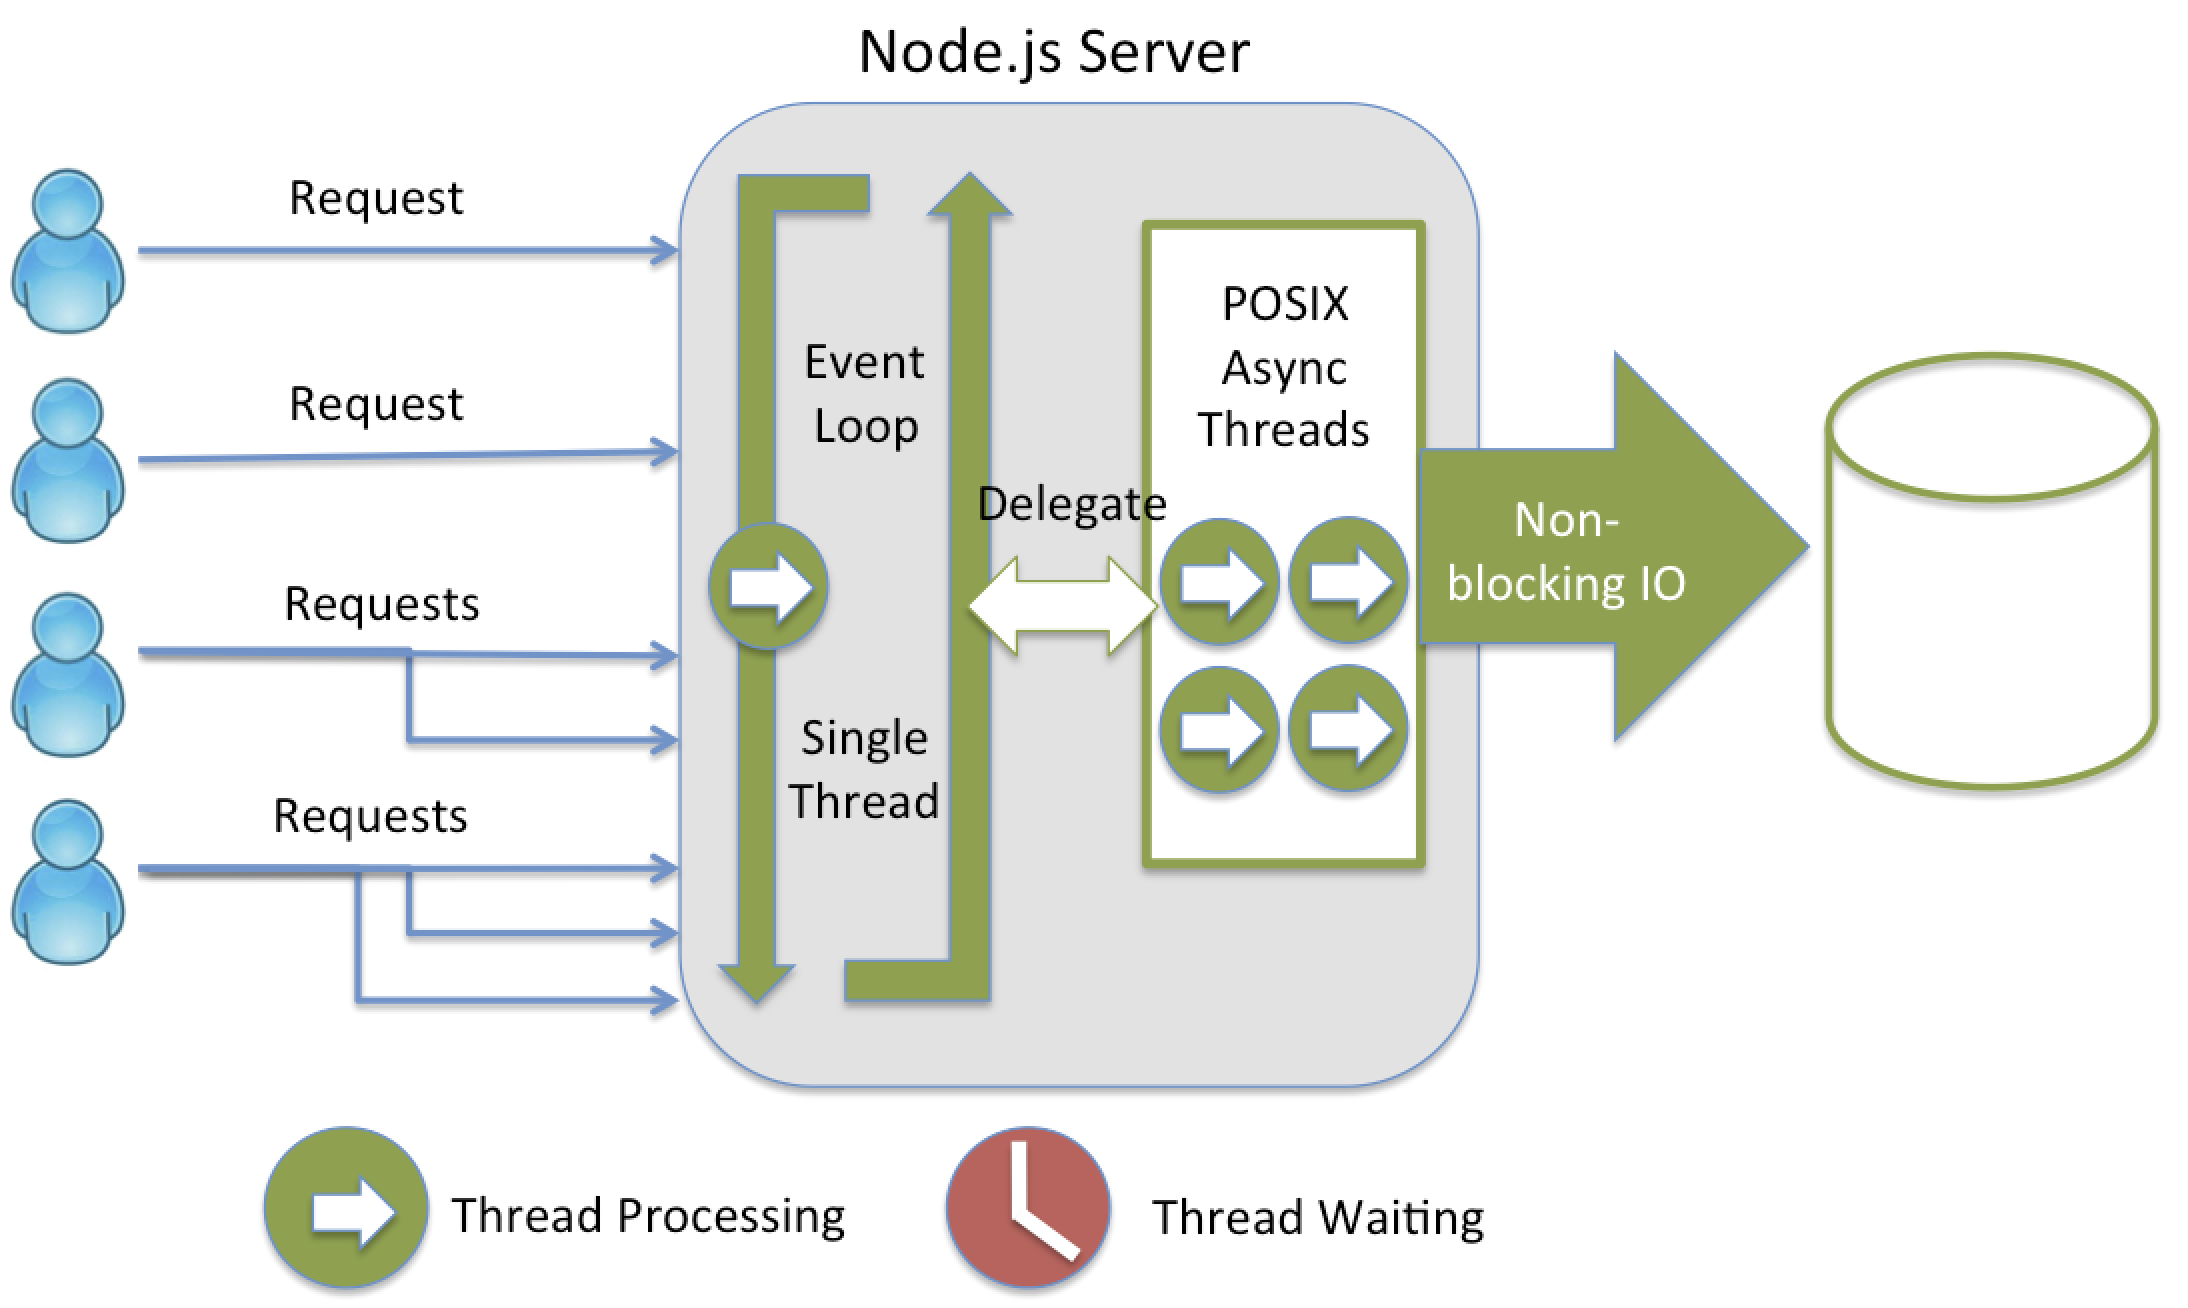
\includegraphics[width=0.6\textwidth]{figures/node.png}
\caption{NodeJS's event driven achitecture.\label{fig:node}}
\end{figure}

\section{Dependent modules}

There are external modules that handle HTTP requests, creates responses and read JSON data. There is also a database connector for Stardog. 

The ExpressJS module acts as the Servler engine for JavaScript. It handles incomming connections and parsed HTTP request are passed to a callback function which generates the responses. Different urls can have different callback functions to do routing. Express also supports many templating engines. EJS is a popular, easy to understand templating engine that was chosen for the project.

Restler is an easy to use module that can asynchronously read a web page and parse it as JSON data and return it to the callback function. This can be used to communicate with the SOS server.

Stardog.JS is Stardog database servers own connector to get SPARQL queries. It is in early stages, however all the necessary functions are working. 

Nodemon is a utility that runs JavaScript codes automatically restarts them on error or code changes. This makes development easier, because every time the source is changed the application automatically restarts. It can be configured to restart on errors to make applications fail safe.

AngularJS is not a server side module, but plays a very important role in the software. This tool is for the browser and it puts a MVC layer on top of the webpage. With the help of Angular, parts of a page can be changed asynchronously based on the value read from the model. It makes the pageload faster by firstly loading the frame of the application and only later inserting the read data from the database. Angular is maintained by Google and it is used in many of their web applications.

\section{RDF representation of the SOS data}

The meta information and the procedure id of an SOS sensor has to be stored in the RDF database to build a semantic representation on top of it. Although a transparent transformation is ready to create RDF XML files from SOS data export, the hierarchy of the sensors is still varying. There are two different approaches.

The first one is to create a tree on top of the sensors manually to describe the connections between each sensor. This often needs to be changed when new sensors arrive in the system. However, this tree can be exported and shared with others just like DBPedia ontologies. This can be also efficiently queried.

The second approach is to use a less redundant way by only creating rules that make sensors part of groups. These rules add a virtual groups based on the conditions defined. This is a resource intensive process that has to be re-run at every query. 

For the experiment the first way is used on a small sample ontology. The hierarchy was manually created and some properties have been added. These properties were annotated as filterable or observable. Observable meaning that the property can be seen from the monitoring system and filterable meaning that its value can be given to advance the query. The structure of the translation is not as straight forward as the created database, however it can be represented in the same way using rules. 

\section{Using the RDF database}

To connect to the database the Stardog.js library has been used. The statically retrieved web page asynchronously requested the list API call to get a list of the filterable properties and their range. The ranges can be either other entities, doubles, integers or strings. Depending on what the range of the property is a corresponding input box shall be rendered.

When the AJAX call responds the Angular script reloads the data with the response. 

On the backend a separate module handles the API calls, connects to the database and runst the SPARQL request. The result and additional information is returned as JSON response.

% TODO: SPARQL queries, sequence diagram, etc.

\section{Connecting the SOS server}

The JSON API can be reached easily using the Restler module to retrieve information from the SOS server. The server responds to the GetCapabilities queries with its list of the sensors and their parameters. However, yet there has not been progress in implementing the GetObservation command in the JSON interface. The JSON API is still under heavy development, thus further connection using this interface can not be done.

\section{Solving the challenge}

To solve the issue of connecting to the JSON interface there can be three different ways. 

The first one is to connect to the SOS server using another interface. There are SOAP interfaces implemented for NodeJS, by adding this layer the GetObservation method can be queried.

The second method is to implement the GetObservation method in the 52north SOS server. The development environment has been already set up, after examining the code the changes shoul be made easily. 

Because of the many changes that are needed to display SOS data changing to an existing SOS client should be a great step forward. The existing client can be extended by semantic functions using the Stardog library provided and the some SPARQL queries. The development environment for the SWE Client is also ready to use.

\section{Using the Software}

Thanks to NodeJS package management the software is easy to deploy. After installing NodeJS - in Windows there is a straight-forward installer, for Ubuntu it can be easily installed using apt - the git project has to be cloned to the server. In the project directory (sensormonitor)  the npm install command installs the missing modules and the npm start command starts the application with Nodemon. The url of the rdf database can be changed in rdf\_parser.js. The installation commands are shown on listing \ref{lst:install}

\begin{lstlisting}[caption={Install steps for the software\label{lst:install}}]
#0. install NodeJS and npm
sudo apt-get install nodejs
#1. clone the project to your destination
git clone --depth 1 https://djlancelot@bitbucket.org/djlancelot/sensormonitor.git
#2. change into project folder
cd sensormonitor
#3. install missing dependencies
npm install
#4. start the application
npm start
\end{lstlisting}